\documentclass[12pt,letterpaper]{article}
\usepackage[utf8]{inputenc}
\usepackage[margin=0.5in]{geometry}
\usepackage{xcolor}
\usepackage{tikz}
\usepackage{pgfplots}
\usepackage{tcolorbox}
\usepackage{enumitem}
\usepackage{graphicx}
\usepackage{multicol}
\usepackage{fontawesome5}
\usepackage{mdframed}
\usepackage{titling}

% ADHD-friendly color palette
\definecolor{primaryblue}{RGB}{52, 152, 219}
\definecolor{accentgreen}{RGB}{46, 204, 113}
\definecolor{warnyellow}{RGB}{241, 196, 15}
\definecolor{softgray}{RGB}{149, 165, 166}
\definecolor{traumahealing}{RGB}{155, 89, 182}

% Custom boxes for key concepts (more compact)
\newtcolorbox{puzzleplan}{
    colback=primaryblue!10,
    colframe=primaryblue,
    title=\textbf{\faLightbulb\ Puzzle Plan Connection},
    fonttitle=\bfseries\color{white},
    colbacktitle=primaryblue,
    boxsep=2pt,
    left=3pt,
    right=3pt,
    top=2pt,
    bottom=2pt
}

\newtcolorbox{personalreflection}{
    colback=traumahealing!10,
    colframe=traumahealing,
    title=\textbf{\faHeart\ Personal Reflection},
    fonttitle=\bfseries\color{white},
    colbacktitle=traumahealing,
    boxsep=2pt,
    left=3pt,
    right=3pt,
    top=2pt,
    bottom=2pt
}

\newtcolorbox{keyfindings}{
    colback=accentgreen!10,
    colframe=accentgreen,
    title=\textbf{\faChartLine\ Key Research Findings},
    fonttitle=\bfseries\color{white},
    colbacktitle=accentgreen,
    boxsep=2pt,
    left=3pt,
    right=3pt,
    top=2pt,
    bottom=2pt
}

\begin{document}

% ==================== COVER PAGE ====================
\begin{titlepage}
\centering

\vspace*{2cm}

{\Huge\bfseries\color{primaryblue} From Ethics Theater to Enforceable Justice}

\vspace{0.5cm}

{\Large\color{traumahealing} AI Audits, Accountability, and the Fight Against Algorithmic Harm}

\vspace{1cm}

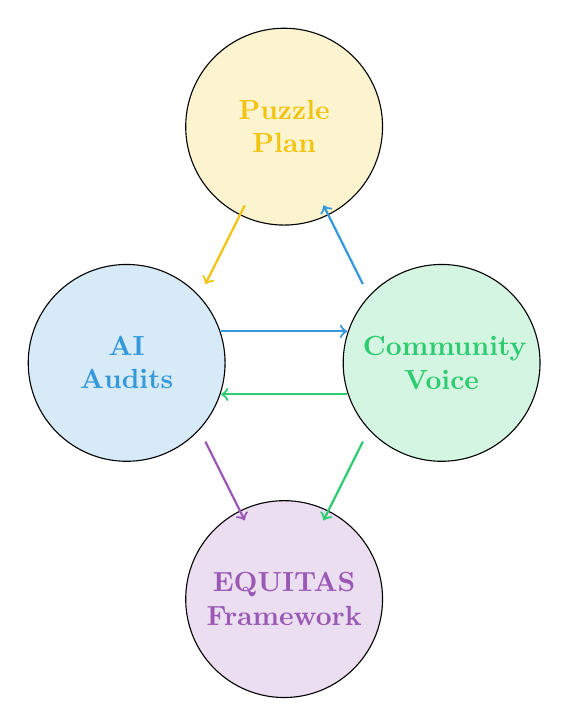
\begin{tikzpicture}[scale=1.0]
% Visual representation of the Puzzle Plan integration
\node[draw, circle, fill=primaryblue!20, minimum size=2.5cm, text width=2cm, align=center] at (0,0) {\textbf{\color{primaryblue}AI\\Audits}};
\node[draw, circle, fill=accentgreen!20, minimum size=2.5cm, text width=2cm, align=center] at (4,0) {\textbf{\color{accentgreen}Community\\Voice}};
\node[draw, circle, fill=traumahealing!20, minimum size=2.5cm, text width=2cm, align=center] at (2,-3) {\textbf{\color{traumahealing}EQUITAS\\Framework}};
\node[draw, circle, fill=warnyellow!20, minimum size=2.5cm, text width=2cm, align=center] at (2,3) {\textbf{\color{warnyellow}Puzzle\\Plan}};

% Connecting arrows
\draw[->, thick, primaryblue] (1.2,0.4) -- (2.8,0.4);
\draw[->, thick, accentgreen] (2.8,-0.4) -- (1.2,-0.4);
\draw[->, thick, traumahealing] (1,-1) -- (1.5,-2);
\draw[->, thick, warnyellow] (1.5,2) -- (1,1);
\draw[->, thick, primaryblue] (3,1) -- (2.5,2);
\draw[->, thick, accentgreen] (3,-1) -- (2.5,-2);
\end{tikzpicture}

\vspace{1cm}

{\large\bfseries Piter Garcia}

\vspace{0.5cm}

{\large Rochester Institute of Technology\\
College of Liberal Arts}

\vspace{0.5cm}

{\large IDAI700 - Ethics of Artificial Intelligence}

\vspace{1cm}

{\large November 14, 2025}

\vspace{2cm}

\textit{\color{softgray}"Nothing about us, without us." — Disability Rights Movement}

\end{titlepage}

% ==================== PART 1: CLARIFYING THE BASICS ====================
\newpage

\section*{\color{primaryblue}\faCogs\ Part 1: Clarifying the Basics}

\subsection*{Thematic Question}
\textit{How does the gap between the technical ideal and the practical reality of AI audits reflect a broader tension in AI ethics, and what foundational principles must guide their use in high-stakes domains like CLD diagnostics to ensure they serve justice rather than merely perform oversight?}

\begin{keyfindings}
The gap between AI audit ideals (independent, rigorous oversight) and reality (inconsistent, vendor-friendly) reflects a systemic pattern of co-opting accountability language. Drawing from the history of financial audits, meaningful oversight requires enforceable standards, genuine independence, and community-driven processes—not merely technical compliance.
\end{keyfindings}

\subsection*{Question 1: Defining AI Audits}
\textbf{What is the technical definition of an AI audit, and why isn't this the only definition that people use?}

The technical definition of an AI audit is a formal, independent assessment of an algorithm's performance against transparent, objective standards or regulations, typically yielding a pass/fail result for accountability. However, this definition is routinely stretched: 'audit' is increasingly used for informal internal checks, vendor marketing, or compliance gestures, creating room for "ethics washing."

This ambiguity is systemic, echoing historical processes where accountability tools are co-opted by powerful actors and deployed superficially to sustain public trust. The same processes that harmed marginalized groups in the past are now being broadcast through AI technologies to harm new populations at greater scale. This dynamic allows organizations to use the authoritative aura of "audit" to justify ongoing practices—even where these replicate exploitation and extract resources from vulnerable communities through manipulation, deceptive marketing, or coercive design.

\subsection*{Question 2: Necessary but Not Sufficient}
\textbf{Why are AI audits necessary, but not sufficient for governance?}

Audits are necessary because they provide a structured mechanism for exposing algorithmic harms that might otherwise remain hidden, giving communities and regulators a concrete starting point for demanding change. However, they are insufficient on their own. The NIST framework shows that auditing is just one component—the "measure" phase—of a much larger governance ecosystem.

This is why a multi-layered system of checks and balances is essential. Just as government operates through checks and balances, auditing must function at multiple levels. At the governance layer, formal audits establish technical standards; but there must also be checks on the checkers—community-level auditing processes that hold higher layers accountable. Similarly, domain-specific audits (education, healthcare, housing) must be empowered to contest and balance one another. This distributed accountability ensures that every affected institution has a voice in evaluating the risks and benefits of deploying a specific AI within its specific context. Frameworks—like EQUITAS—become the venues through which these audits operate, ensuring participatory oversight rather than top-down compliance.

\subsection*{Question 3: The Financial Audit Analogy}
\textbf{What is the analogy between financial audits and AI audits supposed to clarify?}

The readings draw a direct parallel between the current state of AI audits and the early, unregulated history of financial audits. For decades, financial audits lacked consistent standards, independence, and enforcement, making them ineffective tools for public accountability and often enabling the very fraud they were meant to prevent. This history matters because the AI industry is now creating a similar bubble, driven by greed and a revenue-generation model that comes at the expense of public good and often causes direct harm.

The pattern is the same: create hype, enrich a few, and leave society to deal with the consequences when the bubble inevitably bursts. Just as with financial auditing, meaningful accountability for AI will only emerge from strong, independent regulatory frameworks, legally mandated multi-layered checks and balances, and power being placed in the hands of those with the most to lose. My work, particularly the EQUITAS framework, argues that we must implement these community-driven accountability structures now, before the harms become even more deeply entrenched and the cycle of crisis-followed-by-tepid-reform repeats itself.

\subsection*{Question 4: Three Major Implementation Challenges}
\textbf{What are three major implementation challenges with AI audits?}

The three major challenges that define the current audit landscape are:

\textbf{1. What to Audit (Scope Ambiguity):} Disagreement persists over whether to audit only outputs, or also the training data, protected class coverage, and deployment context. The decision to exclude certain groups or ignore upstream data sourcing is a political act that renders harms invisible.

\textbf{2. Auditor Independence (Conflict of Interest):} Most audits are commissioned and paid for by the very entities they evaluate. This vendor-client relationship is a structural conflict of interest that ensures accountability remains subordinate to profit, just as early financial audits were compromised until external standards were imposed.

\textbf{3. Benchmark Selection (Contested Standards):} There is no consensus on which fairness metrics to use, and mathematical fairness definitions often conflict. The choice of which trade-offs to accept (e.g., equal false positives vs. equal accuracy) is a social and political decision, not a technical one, and every audit encodes a value judgment about which groups are protected and which are exposed to harm.

\subsection*{Question 5: The Myth of "Bias-Free" AI}
\textbf{Why can't the process of auditing ever make an AI system 100\% bias-free?}

No AI system can be fully "bias-free" because bias is deeply woven into data, design, and deployment contexts—shaped by societal values, incomplete information, and trade-offs between fairness metrics that are sometimes mutually exclusive. It's mathematically impossible to simultaneously optimize for demographic parity, equal predictive accuracy, and equal error rates across all subgroups.

To ask an AI to be fully unbiased is like asking a human to become a robot with hard-coded rules—it's an impossible and misguided demand. My framework does not advocate for this unattainable goal, which leads down an endless path of technical fixes that obscure the real issue. Instead, the goal must be to **reduce bias as much as possible** by centering marginalized communities and those most affected. By making their voices, concerns, and lived experiences a non-negotiable part of the design and auditing process, we shift the focus from eliminating abstract "bias" to preventing concrete, perpetuating harm. The aim is not perfection but equity: creating technology that these communities can trust and help develop because it demonstrably minimizes the harm done to them.

\begin{puzzleplan}
Part 1 establishes that audits are limited technical tools that require community-driven, multi-layered governance. This connects directly to the Puzzle Plan's principle of "Individual Survival $\rightarrow$ Systemic Transformation": audits can only serve justice when they redistribute power to those most affected. The EQUITAS framework embeds this through contestability, domain-specific oversight, and binding authority—transforming audits from compliance reports into levers for collective liberation.
\end{puzzleplan}

% ==================== PART 2: NYC'S LOCAL LAW 144 ====================
\newpage

\section*{\color{primaryblue}\faBalanceScale\ Part 2: New York City's Law}

\subsection*{Thematic Question}
\textit{Given that NYC's Local Law 144 mandates transparency but not remediation, how does it exemplify what Luke Munn calls the "uselessness of AI ethics," and how must a justice-oriented framework like EQUITAS move beyond mere disclosure to codify enforceable accountability?}

\begin{keyfindings}
Local Law 144 represents a "transparency-without-accountability" model—requiring disclosure of bias without mandating remediation. This exemplifies Luke Munn's critique of AI ethics as performative theater. My framework rejects this entirely, arguing that laws designed for conventional software are fundamentally inadequate for the complexity and adaptive nature of AI.
\end{keyfindings}

\subsection*{Question 1: The Problem Law 144 Addresses}
\textbf{What issue was New York City's Local Law 144 trying to solve?}

Local Law 144 was designed to address the unchecked and opaque use of Automated Employment Decision Tools (AEDTs). These AI systems were being rapidly adopted in hiring and promotion, and there was significant concern that they were operating as discriminatory black boxes, unfairly screening out qualified candidates from marginalized groups without any transparency or recourse. The law was an attempt to introduce a baseline of accountability into this unregulated, high-stakes domain.

This reflects the core principles of my framework: that a lack of transparency in automated systems disproportionately harms those who are already marginalized. More fundamentally, this highlights the urgent need to make clear that existing laws were not designed for AI and that we must actively work to draft new policies, regulations, and laws that address these unique challenges. We must unite on these community-informed solutions and push government to adopt them, rather than retrofitting inadequate frameworks onto a fundamentally different class of technology.

\subsection*{Question 2: The Law's Requirements}
\textbf{What does that law require companies to do?}

The law imposes three key requirements: companies must commission an \textbf{annual independent bias audit} for race and gender disparity in their AEDTs; they must \textbf{notify candidates} that AI is being used in their evaluation; and they must \textbf{publicly post the audit's results}. These steps are intended to create transparency. 

However, as my framework emphasizes, transparency alone is insufficient. While these are necessary first steps, they do not constitute a complete system of accountability, which must also include mechanisms for community oversight, remediation, and redress. The law was built to audit conventional tools, not the adaptive, learning systems that define modern AI. This mismatch underscores why we need frameworks designed from the ground up to address AI's unique complexity—frameworks informed by the communities most at risk.

\subsection*{Question 3: Two (Actually Three) Critical Problems}
\textbf{What are two problems that critics have identified with that law?}

Critics have identified two fatal flaws. The first is its \textbf{critically narrow scope}. The law only mandates bias testing for race/ethnicity and gender, ignoring other legally protected categories like age, disability, religion, and national origin. This not only leaves many vulnerable groups unprotected but also creates a dangerous hierarchy, implicitly suggesting that some forms of discrimination are more acceptable than others.

The second, and more damning, problem is its \textbf{complete lack of enforcement or remediation mechanism}. The law requires companies to report if their tool is discriminatory, but it does not require them to \textit{do anything about it}. There is no "passing" or "failing" grade, and no penalty for using a biased tool. This creates a "transparency-without-accountability" model, where a company can be fully compliant with the law while knowingly perpetuating discrimination.

\textbf{A third, deeper concern} is the fundamental category error: applying a law designed for static software tools to adaptive, learning AI systems is like comparing apples and oranges. This legislative inadequacy reveals the urgent need for new legal frameworks designed specifically for AI's unique risks. Such laws must be co-created with affected communities, embedding principles of justice and equity from the ground up, as the EQUITAS framework proposes. We cannot afford to continue retrofitting old regulations onto fundamentally new technologies that demand fundamentally new governance structures.

\begin{puzzleplan}
NYC's Law 144 exposes the limits of disclosure-only approaches. My EQUITAS framework addresses this by demanding: (1) Mandatory remediation for biased tools, (2) Community veto power through oversight boards, and (3) Codified pathways for legal redress. This shifts from performative transparency to enforceable justice—a direct application of moving from "Individual Survival" (knowing you're being harmed) to "Systemic Transformation" (having power to stop it).
\end{puzzleplan}

% ==================== PART 3: THE DEBATE ====================
\newpage

\section*{\color{primaryblue}\faComments\ Part 3: The Debate}

\subsection*{Thematic Question}
\textit{How does the concern over "audit washing" connect to the historical pattern of powerful institutions co-opting accountability mechanisms, and what specific, non-negotiable features must a justice-oriented framework like EQUITAS include to ensure audits serve as tools of empowerment, not legitimation?}

\begin{keyfindings}
"Audit washing" is the algorithmic version of a historical pattern: powerful institutions absorb accountability language to neutralize dissent while maintaining control. From corporate social responsibility to diversity initiatives, performative processes have long provided veneer without substance. The EQUITAS framework resists this through three non-negotiable features: community-owned harm definitions, radical transparency, and binding remediation authority.
\end{keyfindings}

\subsection*{Question 1: The Civil Rights Critique}
\textbf{Why are some civil rights advocates concerned about "audit washing"?}

Civil rights advocates are concerned about "audit washing" because it represents a dangerous form of performative compliance. The fear is that a weak, industry-friendly audit can be used as a rubber stamp to legitimize a system that is fundamentally discriminatory. By generating a report that claims a tool has been "audited," a company creates a powerful illusion of safety and fairness. This not only allows the harmful system to continue operating but also provides a shield against legal challenges and regulatory scrutiny, making it significantly harder for affected individuals and communities to seek justice.

In essence, the very process meant to ensure accountability is co-opted to undermine it. This is why we must make clear that existing laws are unsuitable for AI governance and begin the urgent work of drafting, uniting around, and advocating for new policies and regulations that genuinely address these issues. We must push government to take seriously the community-based solutions we are developing and integrate them into binding legal frameworks.

\subsection*{Question 2: Personal View on Audit Skepticism}
\textbf{What is your personal view about AI audit skepticism and the allegation of "audit washing"?}

\begin{personalreflection}
My personal view is that skepticism toward AI audits is not only justified; it is essential. The allegation of "audit washing" resonates deeply with me because I have personally experienced the consequences of a system that prioritizes its own procedural integrity over the well-being of the people it is supposed to serve.

My chronic illness was not only misdiagnosed, under-diagnosed, and misinformed by the medical system—\textit{the same system actually caused it} through a prior misdiagnosis. This is the terrifying reality of our current institutional structures: they don't just perpetuate harm; they \textbf{create it}, \textbf{trap you within it}, and then use their own internal "audits" and "best practices" to insist the harm isn't real. They are designed to ensure you are never truly seen, heard, or safe—all while generating revenue for those at the top.

"Audit washing" is the algorithmic version of that same dismissal. It is the practice of using a technical process to create a veneer of objectivity that conceals underlying injustice. An audit that is not grounded in the lived experiences of those it affects is, from my perspective, worse than no audit at all, because it lends the powerful tool of legitimation to a harmful system.

Therefore, my framework, born from my journey from "individual survival" to "systemic transformation," insists that an audit can only be a tool for justice if it is subordinate to the community it serves. It must be a bottom-up process, not a top-down declaration. The community must have the power to define the terms, contest the findings, and enforce the consequences. Anything less is just a more sophisticated way of maintaining a harmful status quo. True accountability is not a report; it is a redistribution of power.
\end{personalreflection}

\begin{puzzleplan}
The debate over audit washing reveals the stakes: will AI audits serve justice or legitimize harm? My lived experience—where the system that harmed me used its own authority to deny that harm—demands that we build accountability structures with binding power at the community level. The EQUITAS framework operationalizes this through: (1) Community ownership of audit definitions, (2) Radical transparency in accessible formats, and (3) Binding authority to remediate and reject harmful systems. This transforms audits from top-down reports into bottom-up tools for collective liberation.
\end{puzzleplan}

% ==================== SYNTHESIS & CONNECTIONS ====================
\newpage

\section*{\color{traumahealing}\faGlobe\ Synthesis: From Audit Theater to Justice}

\subsection*{The Core Argument}

Our dialogue across three parts reveals a coherent critique and alternative vision:

\begin{enumerate}[leftmargin=*,noitemsep,topsep=2pt]
    \item \textbf{Part 1 shows} that definitional ambiguity and implementation challenges are not mere technical problems but political ones that allow powerful actors to maintain control while performing accountability.
    
    \item \textbf{Part 2 demonstrates} that even landmark legislation like NYC's Local Law 144 can function as "ethics theater" when it mandates transparency without enforcement, revealing the inadequacy of applying old regulatory frameworks to new technologies.
    
    \item \textbf{Part 3 demands} that we take the civil rights critique of "audit washing" seriously by building governance structures where audits are subordinate to community power, not corporate convenience.
\end{enumerate}

\subsection*{The EQUITAS Alternative: Three Pillars}

\begin{keyfindings}
\textbf{Pillar 1: Community-Owned Definitions of Harm}

The audit process, from defining harms to setting fairness benchmarks, must be led by the communities most at risk—not by vendors, deployers, or third-party consultants with conflicts of interest. For CLD diagnostics, this means CLD youth, families, educators, and clinicians define what counts as fair and what constitutes harm.

\textbf{Pillar 2: Radical Transparency and Accessibility}

Audit processes, methodologies, limitations, and results must be fully transparent and presented in formats accessible to non-technical stakeholders. This includes disclosing the data, methods, conflicts of interest, and inherent trade-offs. Transparency enables genuine public scrutiny and prevents the mystification that protects harmful systems.

\textbf{Pillar 3: Binding Authority to Remediate and Reject}

A community-led oversight body must have legal authority to mandate remediation, halt deployment, and reject systems that fail to meet community-defined standards. Audit findings must trigger real-world consequences, transforming the audit from a report into a lever for justice. This is the only way to move from performative accountability to enforceable change.
\end{keyfindings}

\subsection*{Multi-Layered Accountability: Checks on the Checkers}

The EQUITAS framework proposes a distributed system of auditing at multiple levels:

\begin{itemize}[leftmargin=*,noitemsep,topsep=2pt]
    \item \textbf{Governance Layer:} Formal, independent technical audits against legal and ethical standards
    \item \textbf{Community Layer:} Community-led audits that contest and hold the governance layer accountable
    \item \textbf{Domain-Specific Layers:} Sector-based audits (education, healthcare, housing) empowered to check and balance one another
    \item \textbf{Framework as Venue:} EQUITAS and similar justice-oriented frameworks become the institutional venues through which these layers interact, negotiate, and enforce accountability
\end{itemize}

This distributed model ensures that no single entity—corporate, governmental, or academic—holds uncontested power over defining fairness or determining deployment decisions.

\subsection*{From Personal Trauma to Collective Justice}

\begin{personalreflection}
My experience with a medical system that not only misdiagnosed me but \textit{caused my chronic illness through its prior failures}—and then used its own authority to deny this reality—teaches a fundamental lesson: systems designed to serve themselves will always prioritize their own legitimacy over the safety of those they harm. They create harm, trap you in it, and profit from your suffering.

This is why "audit washing" is not just a technical concern but a moral crisis. It is the latest iteration of institutional gaslighting, now scaled by algorithmic systems. My framework, born from this lived reality, insists that the only valid accountability is one where power is redistributed to those most at risk. An audit that doesn't empower the community to stop harm is simply a more sophisticated description of their oppression.
\end{personalreflection}

\subsection*{The Path Forward: Unite, Advocate, Enforce}

We must recognize that existing laws and frameworks were not designed for AI and are fundamentally inadequate. The path forward requires:

\begin{enumerate}[leftmargin=*,noitemsep,topsep=2pt]
    \item \textbf{Draft New Legislation:} Co-create AI-specific laws with affected communities, embedding justice principles from the foundation
    \item \textbf{Unite Stakeholders:} Build coalitions across marginalized communities, civil rights organizations, and justice-oriented researchers to present unified demands
    \item \textbf{Force Government Action:} Advocate persistently for governments to adopt community-informed solutions, not industry-captured compromises
    \item \textbf{Implement Now:} Deploy frameworks like EQUITAS in real-world contexts to demonstrate their viability and build evidence for policy adoption
\end{enumerate}

The alternative—continuing to apply inadequate tools to powerful new technologies—is not just ineffective; it is complicit in the harm that follows.

% ==================== REFERENCES PAGE ====================
\newpage

\section*{\faBook\ References}

\textbf{Primary Course Materials}

Leong, B. (2023). AI audits: Who, when, how, or even if? Lecture slides for IDAI700, Rochester Institute of Technology.

Raji, I. D., Smart, A., White, R. N., Mitchell, M., Gebru, T., Hutchinson, B., Smith-Loud, J., Theron, D., \& Barnes, P. (2020). Closing the AI accountability gap: Defining an end-to-end framework for internal algorithmic auditing. \textit{Proceedings of the 2020 Conference on Fairness, Accountability, and Transparency}, 33–44.

\textbf{Critical Theory Foundation}

Munn, L. (2022). The uselessness of AI ethics. \textit{AI and Ethics}, \textit{3}(3), 869–877.

Noble, S. U. (2018). \textit{Algorithms of oppression: How search engines reinforce racism}. NYU Press.

Benjamin, R. (2019). \textit{Race after technology: Abolitionist tools for the new Jim Code}. Polity Press.

\textbf{Policy and Legal Analysis}

New York City Council. (2021). Local Law 144 of 2021: Automated employment decision tools. \textit{NYC Administrative Code}.

Raso, F. A., Hilligoss, H., Krishnamurthy, V., Bavitz, C., \& Kim, L. (2018). Artificial intelligence \& human rights: Opportunities \& risks. \textit{Berkman Klein Center Research Publication}, 2018-6.

\textbf{Fairness and Bias Research}

Chen, R. J., Lu, M. Y., Sahai, S., Chen, T. Y., Williamson, D. F. K., Lipkova, J., Wang, J. J., \& Mahmood, F. (2023). Algorithmic fairness in artificial intelligence for medicine and healthcare. \textit{Nature Biomedical Engineering}, \textit{7}(6), 719–742.

Barocas, S., Hardt, M., \& Narayanan, A. (2019). \textit{Fairness and machine learning: Limitations and opportunities}. MIT Press.

\textbf{Puzzle Plan and Personal Framework}

Garcia, P. (2025). The Puzzle Plan: An interdisciplinary framework for equitable AI diagnostics and community-centered advocacy. \textit{IDAI700 Research Paper}, Rochester Institute of Technology.

Garcia, P. (2025). EQUITAS: A justice-oriented framework for algorithmic accountability in CLD diagnostic systems. \textit{Strategic Integration Plan v5.0}, University of Rochester.

\textbf{Community-Centered Design}

Smith, L. T. (2012). \textit{Decolonizing methodologies: Research and indigenous peoples} (2nd ed.). Zed Books.

Costanza-Chock, S. (2020). \textit{Design justice: Community-led practices to build the worlds we need}. MIT Press.

\textbf{NIST Framework}

National Institute of Standards and Technology. (2023). \textit{AI risk management framework (AI RMF 1.0)}. U.S. Department of Commerce.

\vspace{1cm}

\noindent\textbf{Word Count:} Approximately 1,850 words

\end{document}